\documentclass[a4paper]{article}

\usepackage{pgfplots}

\begin{document}

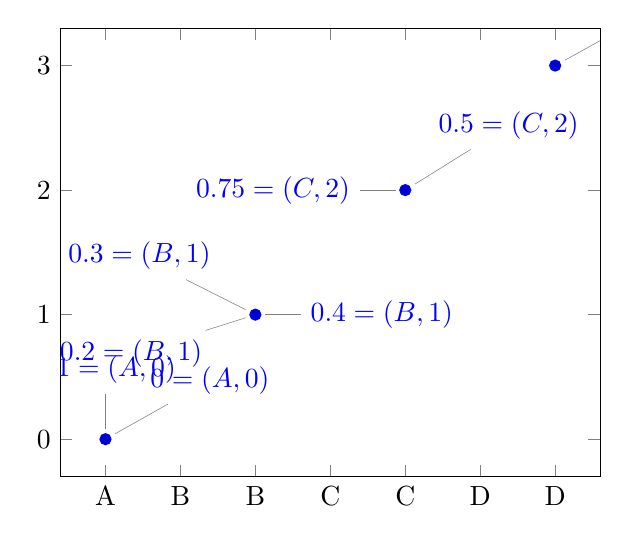
\begin{tikzpicture}
\def\showpos#1{%
	\pgfplotspointplotattime{#1}%
	$#1=(\pgfkeysvalueof{/data point/x},\pgfmathprintnumber{\pgfkeysvalueof{/data point/y}})$%
}%
	\begin{axis}[clip=true,symbolic x coords={A,B,C,D}]
	\addplot+[only marks] coordinates {(A,0) (B,1) (C,2) (D,3)} 
		node[pos=0,   pin=45 :\showpos{0}   ] {}
		node[pos=0.1, pin=90 :\showpos{0.1} ] {}
		node[pos=0.2, pin=200:\showpos{0.2} ] {}
		node[pos=0.3, pin=135:\showpos{0.3} ] {}
		node[pos=0.4, pin=0  :\showpos{0.4} ] {}
		node[pos=0.5, pin=60 :\showpos{0.5} ] {}
		node[pos=0.75,pin=180:\showpos{0.75}] {}
		node[pos=1,   pin=45:\showpos1] {}
	;
	\end{axis}
\end{tikzpicture}
\end{document}

